% Copyright 2004 by Till Tantau <tantau@users.sourceforge.net>.
%
% In principle, this file can be redistributed and/or modified under
% the terms of the GNU Public License, version 2.
%
% However, this file is supposed to be a template to be modified
% for your own needs. For this reason, if you use this file as a
% template and not specifically distribute it as part of a another
% package/program, I grant the extra permission to freely copy and
% modify this file as you see fit and even to delete this copyright
% notice. 

\documentclass{beamer}

\usepackage[utf8]{inputenc}
% \usepackage[cp1250]{inputenc} %% NASTAVENI PRO WINDOWS
% \usepackage[T1]{fontenc} %% puvodni evropske fonty->spatne umistene hacky nad c, d s hackem ma za sebou mezeru
\usepackage[IL2]{fontenc} %fonty vyladene pro cestinu/slovenstinu
\usepackage{booktabs}

% There are many different themes available for Beamer. A comprehensive
% list with examples is given here:
% http://deic.uab.es/~iblanes/beamer_gallery/index_by_theme.html
% You can uncomment the themes below if you would like to use a different
% one:
%\usetheme{AnnArbor}
%\usetheme{Antibes}
%\usetheme{Bergen}
%\usetheme{Berkeley}
%\usetheme{Berlin}
%\usetheme{Boadilla}
%\usetheme{boxes}
%\usetheme{CambridgeUS}
%\usetheme{Copenhagen}
%\usetheme{Darmstadt}
%\usetheme{default}
%\usetheme{Frankfurt}
%\usetheme{Goettingen}
%\usetheme{Hannover}
%\usetheme{Ilmenau}
%\usetheme{JuanLesPins}
%\usetheme{Luebeck}
\usetheme{Madrid}
%\usetheme{Malmoe}
%\usetheme{Marburg}
%\usetheme{Montpellier}
%\usetheme{PaloAlto}
%\usetheme{Pittsburgh}
%\usetheme{Rochester}
%\usetheme{Singapore}
%\usetheme{Szeged}
%\usetheme{Warsaw}

\title[Doking ligandu do tunelu v proteinu]{Automatický doking ligandu do tunelu v proteinu}

% A subtitle is optional and this may be deleted
\subtitle{Diplomová práce}

\author{Jan Plhák}
% - Give the names in the same order as the appear in the paper.
% - Use the \inst{?} command only if the authors have different
%   affiliation.

\date{}
% - Either use conference name or its abbreviation.
% - Not really informative to the audience, more for people (including
%   yourself) who are reading the slides online

\subject{Automatický doking ligandu do tunelu v proteinu}
% This is only inserted into the PDF information catalog. Can be left
% out. 

% If you have a file called "university-logo-filename.xxx", where xxx
% is a graphic format that can be processed by latex or pdflatex,
% resp., then you can add a logo as follows:

% \pgfdeclareimage[height=0.5cm]{university-logo}{university-logo-filename}
% \logo{\pgfuseimage{university-logo}}

% Delete this, if you do not want the table of contents to pop up at
% the beginning of each subsection:

\newcommand{\Rbb}{\mathbb{R}}
\newcommand{\Tau}{\mathrm{T}}


% Let's get started
\begin{document}

\begin{frame}
  \titlepage
\end{frame}

\begin{frame}{Outline}
  \tableofcontents
  % You might wish to add the option [pausesections]
\end{frame}

% Section and subsections will appear in the presentation overview
% and table of contents.
\section{Motivace}
\subsection{Interakce proteinu s ligandem}
\begin{frame}{Interakce proteinu s ligandem}
  \begin{itemize}
  \item {
    \textit{Ligand} je typicky malá molekula, která se na \textit{protein} váže  v jeho \textit{aktivním místě}.
    }
    
  \item {
      Ligandem může být například
      \begin{itemize}
     		\item léčivo, které inhibuje místo v proteinu, které umožňuje viru napadnout buňku.
     		\item substrát, který je při enzymatické reakci přeměněn na produkt (likvidace nebezpečné látky jako je třeba yperit).
     \end{itemize}
  }
  
  \item {
  		Simulace navázání ligandu (vznik stabilního komplexu v aktivním místě) - značná úspora peněz, zrychlení vývoje
  }
  \end{itemize}
\end{frame}


\begin{frame}{Problém}
  \begin{itemize}
  \item {
    	Molekulární doking se používá pro nalezení energetického minima v aktivním místě.
    }
  \item Čím nižší energie, tím vyšší pravděpodobnost, že dojde ke vzniku stabilního komplexu.
  \item {
    	Aktivní místo je ale občas hluboko uvnitř molekuly a ligand musí projít tzv. \textit{tunelem}.
    }
    \item {
    	Pokud tunel obsahuje nějakou silnou energetickou bariéru, ligand jím pravděpodobně neprojde.
    }
    \item {
    	Hledáme spojitou trajektorii ligandu skrze tunel o co nejnižší energii.
    }
  \end{itemize}
\end{frame}

\begin{frame}{Příklad tunelu}
    \begin{figure}
        \includegraphics[width=0.6\textwidth]{img/tunnels.jpg}
    \end{figure}
\end{frame}

\subsection{Výpočet spojité trajektorie}
\begin{frame}{Výpočet spojité trajektorie}
  \begin{itemize}
  \item  V rámci ÚVT a LL vzniká software CaverDock, který bude schopen analyzovat cestu ligandu skrze tunel na základě molekulárního dokingu. Pro jeho fungování je potřeba zajistit diskretizaci tunelu - stěžejní téma této práce.
  \item Diskretizace tunelu - posloupnost omezujících podmínek - řezů.
 	\item Ligand iterativně dokujeme na po sobě jdoucí řezy - simulace procesu navázání a uvolnění ligandu
 	\item Dbáme na to, aby pohyb ligandu tunelem byl spojitý.
  \end{itemize}
\end{frame}

\section{Diskretizační algoritmus}

\begin{frame}{Diskretizační algoritmus}{Vstup a výstup}
\begin{itemize}
	\item Vstup algoritmu - tunel modelovaný posloupností koulí.
	\item Výstup algoritmu - posloupnost řezů, které od sebe nejsou vzdáleny o více než zadaný parametr $ \delta $, neprotínají se ve více než jednom bodě a pokrývají celý tunel.
\end{itemize}

\begin{block}{Definice řezu}
Řezem tunelu $ \Tau $ rozumíme kruh v prostoru, který je určen uspořádanou trojicí
$\theta = (A, u, r)$, kde $ A $ je střed, $ u \in \Rbb^3 $ je normálový vektor a $ r > 0 $ je poloměr.
Pro tento kruh $ \theta $ musí platit, že $ \Tau \cap \theta $ je souvislá množina a navíc
$ \exists \delta > 0 $ tak, že $ \forall \varepsilon > 0,  \varepsilon < \delta $ je
$ (A, u, r + \varepsilon) \cap \Tau = \theta \cap \Tau $.
(Alternativně řečeno $\Tau \setminus \theta $ má dvě komponenty souvislosti.)
\end{block}

\end{frame}

\begin{frame}{Diskretizační algoritmus}{Ukázka diskretizace}
    \begin{figure}
        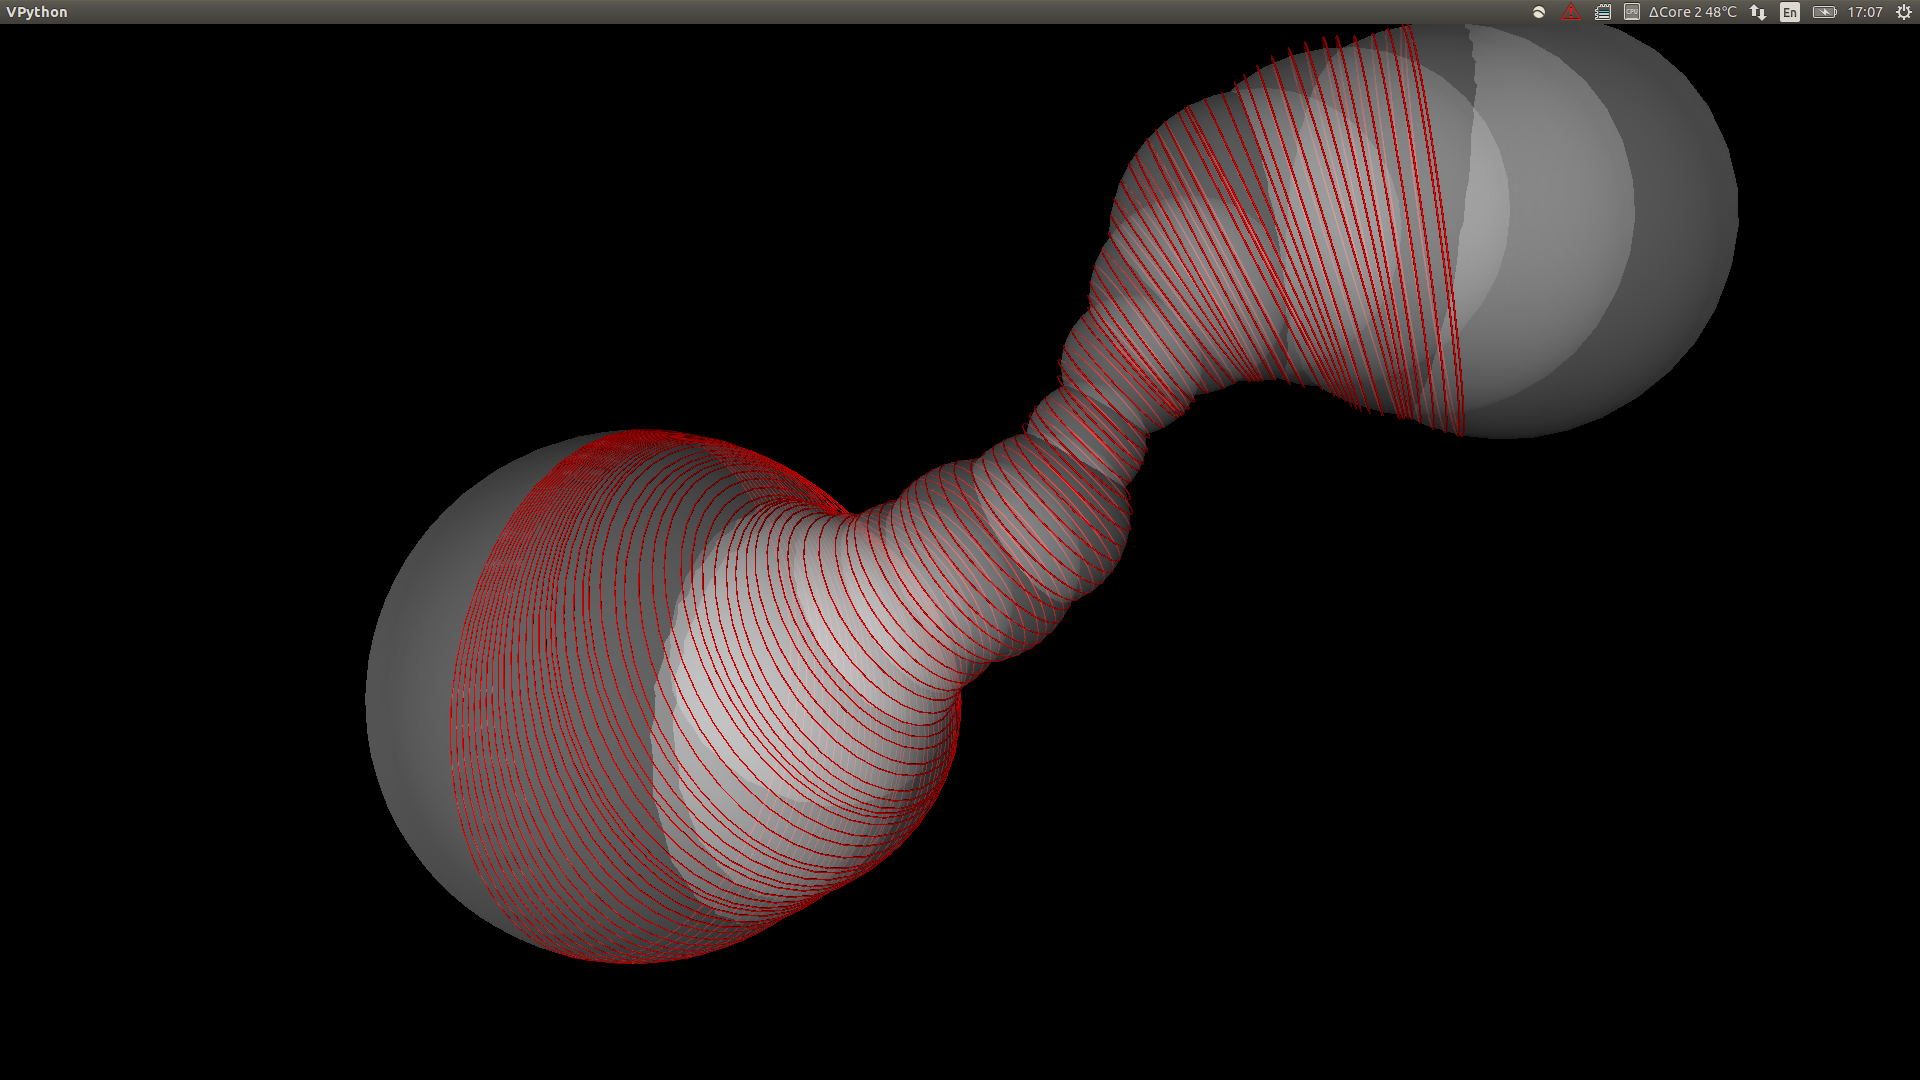
\includegraphics[width=0.9\textwidth]{img/weighted_dir.png}
    \end{figure}
\end{frame}

\begin{frame}{Diskretizační algoritmus}
    \begin{itemize}
	\item Výsledný algoritmus je heuristika - může selhat, avšak pokud skončí, pak je výsledná diskretizace korektní.
	\item Algoritmus byl implementován v jazyce Python.
	\item Testováno na 152 různých tunelech, diskretizace byla vždy nalezena.
	\end{itemize}
\end{frame}

\begin{frame}{Diskretizační algoritmus}{Složitější tunel}
    \begin{figure}
        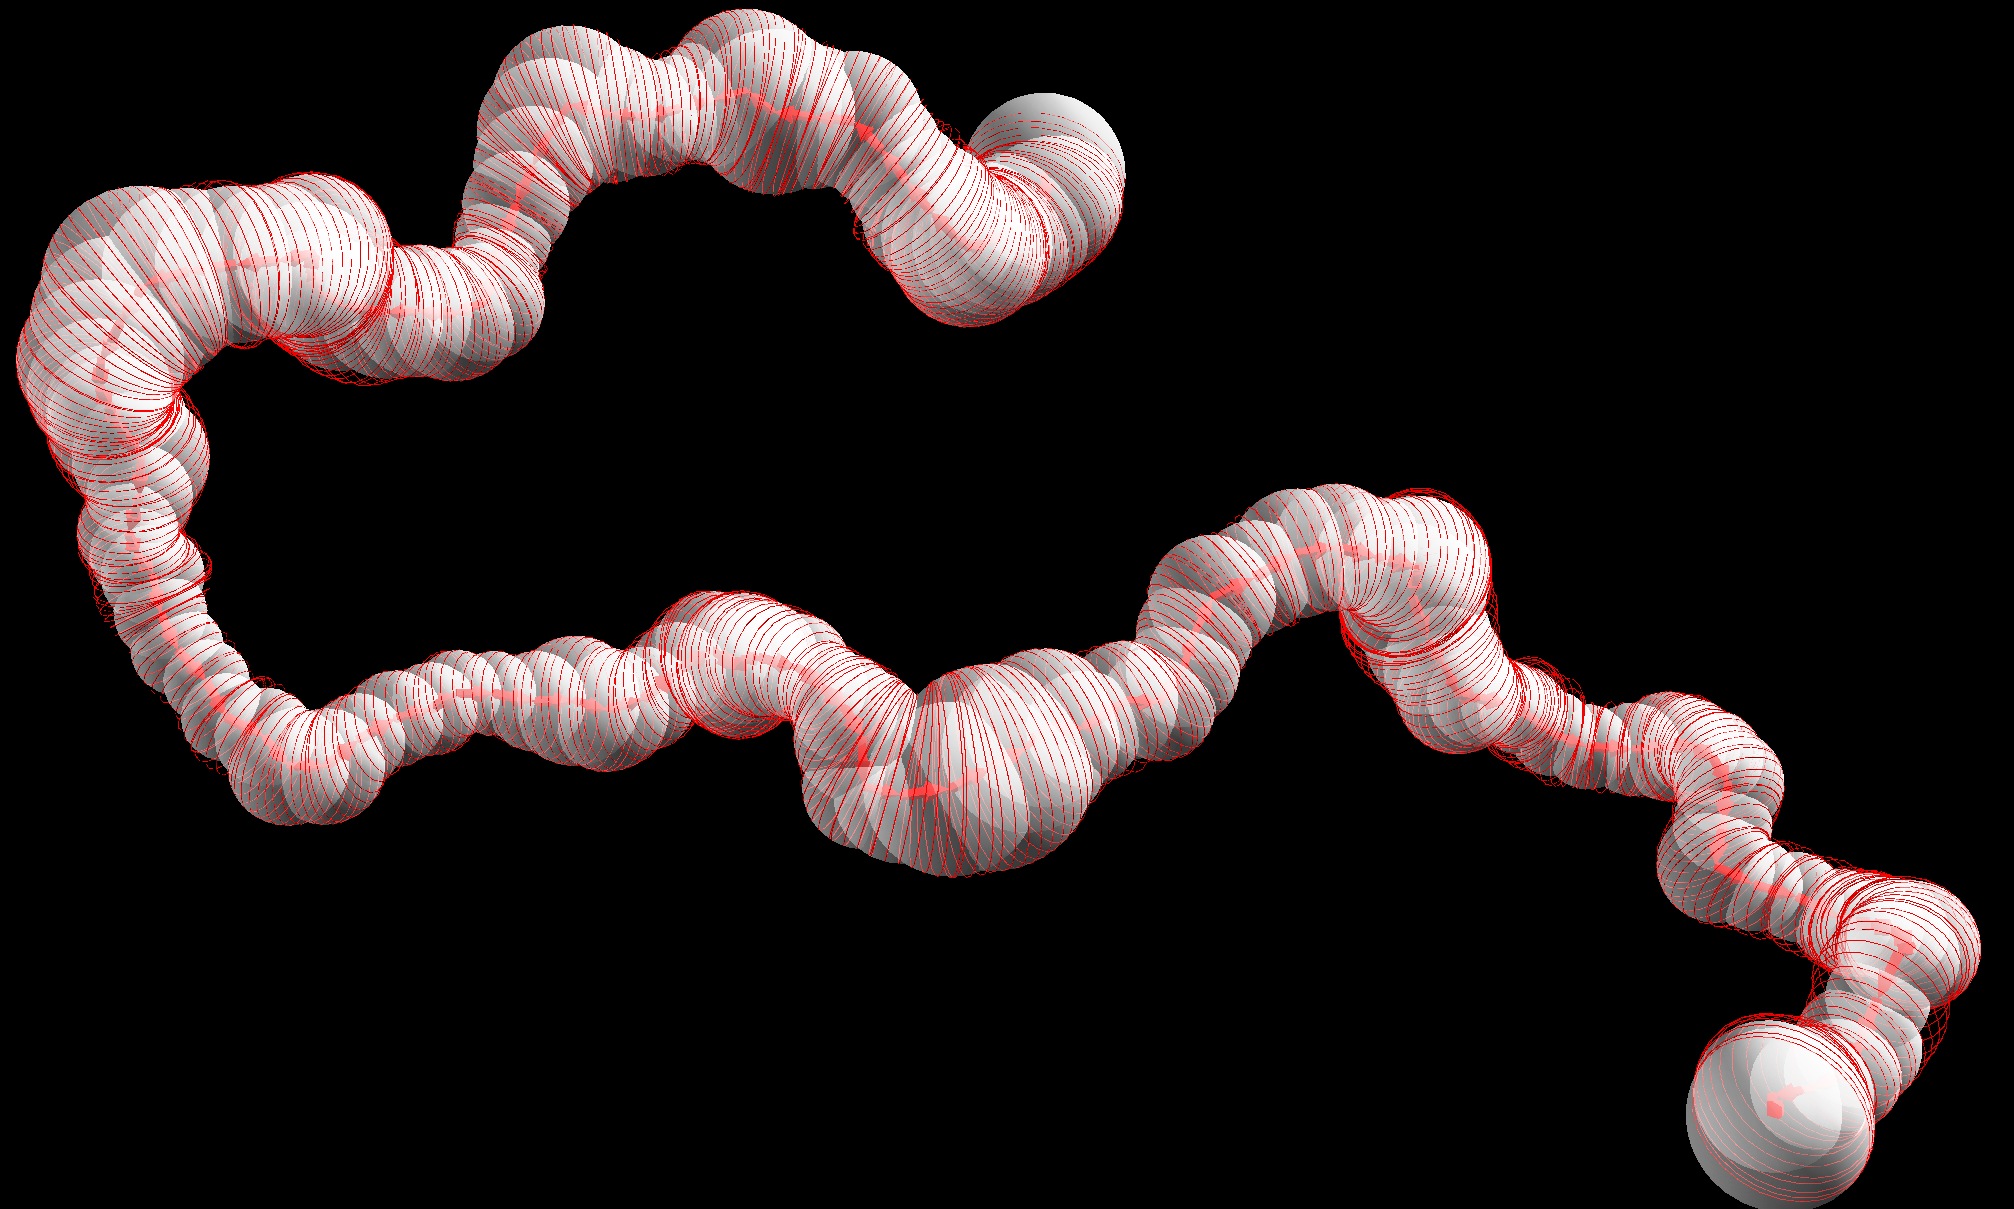
\includegraphics[width=\textwidth]{img/1YGE.png}
    \end{figure}
\end{frame}


\section{Konvergenční algoritmus}
\begin{frame}{Konvergenční algoritmus}
    \begin{itemize}
    \item Tunelem postupujeme dopředným směrem. Pokud narazíme na energetickou bariéru, najdeme konformaci s menší energii a spustíme backtracking.
	\item V případě backtrackingu potřebujeme navázat na dopřednou trajektorii - konvergenční algoritmus.
	\item Optimalizace algoritmu pro hledání spojité trajektorie (potenciálně časová, ale zejména kvalitativní - dosahujeme nižších energií).
	\item Vstup - Molekula proteinu společně s diskretizovaným tunelem, výchozí (dopředná) a cílová (backtracking) konformace ligandu
	\item Výstup - Spojitá posloupnost konformací ligandu, která transformuje výchozí konformaci na cílovou.
	\end{itemize}
\end{frame}

\begin{frame}{Konvergenční algoritmus}{Ilustrace}
    \begin{figure}
        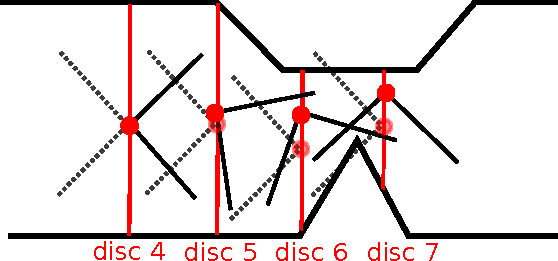
\includegraphics[width=\textwidth]{img/backtracking_bad_rotation.pdf}
        \caption{Obrázek zachycuje situaci, ve které při backtrackingu dojde k opačné
rotaci ligandu.
Dopředná trajektorie je vyznačena tečkovaně, backtracking plnou čárou.
}
    \end{figure}
\end{frame}

\begin{frame}{Konvergenční algoritmus}{Evaluace}
    \begin{itemize}
	\item Algoritmus byl implementován v jazyce C++ a byl začleněn do již existujícího CaverDock softwaru.
	\item V souladu s našimi předpoklady byl přínos konvergenčního algoritmu největší v případě
tunelů s více úzkými hrdly a při počítání s většími ligandy
	\end{itemize}
\end{frame}

\begin{frame}{Konvergenční algoritmus}{Ilustrace}
    \begin{figure}
        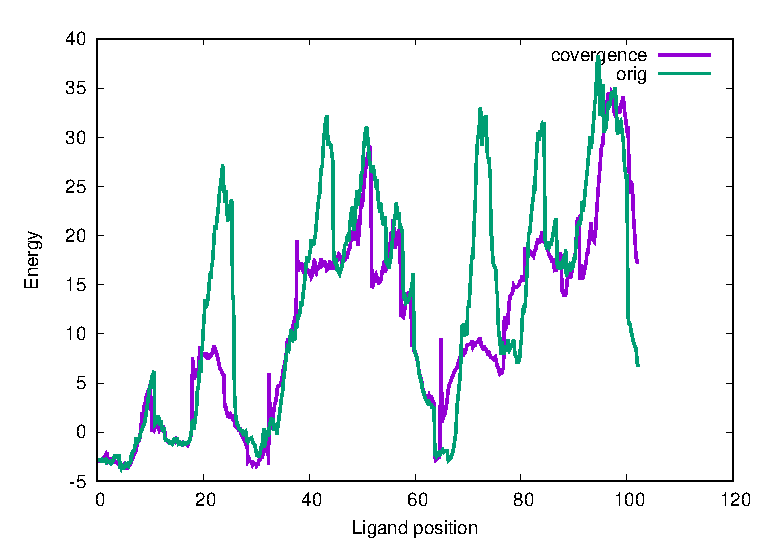
\includegraphics[width=0.7\textwidth]{img/1YGE_energy_m007.eps}
        \caption{Energetický profil v molekule 1YGE pro ligand s 8 atomy a 5 torzními úhly.}
    \end{figure}
\end{frame}

% Placing a * after \section means it will not show in the
% outline or table of contents.
\section*{Summary}

\begin{frame}{Shrnutí}
  \begin{itemize}
  \item
    Návrh a implementace diskretizačního algoritmu.
  \item
    Návrh, implementace a integrace konvergenčního algoritmu a implementace slabého omezujícího vzoru.
    \item V přípravě jsou dva články - biochemický a informatický.
    \end{itemize}
\end{frame}

\begin{frame}
\centering \Large
  \emph{Děkuji za Vaši pozornost.}
  \end{frame}


% All of the following is optional and typically not needed. 
\appendix
\section<presentation>*{\appendixname}
\subsection<presentation>*{Evaluační tabulka}

\begin{frame}{Evaluační tabulka konvergenčního algoritmu}
  \begin{table}[ht]
    \centering
    \begin{tabular}{cccccc}
    \toprule
        & & \multicolumn{2}{c}{Max Energy} & \multicolumn{2}{c}{Avg Energy} \\
        Atoms & DOFs & Orig & Conv & Orig & Conv \\
        \midrule
            2 & 0 & 7.90  &8.00 & 2.94 & 2.95 \\
            3 & 0 & 13.00 & 13.20 & 5.67 & 5.55 \\
            4 & 1 & 20.60 & 19.10 & 7.24 & 7.09 \\
            5 & 2 & 29.70 & 22.20 & 8.99 & 8.34 \\
            6 & 3 & 29.00 & 18.70 & 11.93 & 9.98 \\
            7 & 0 & 41.10 & 41.70 & 21.74 & 21.19 \\
            7 & 4 & 34.10 & 28.20 & 13.50 & 11.14 \\
            8 & 5 & 38.70 & 35.50 & 14.48 & 13.20 \\
            9 & 6 & 49.50 & 42.60 & 17.49 & 15.93 \\
        \bottomrule
    \end{tabular}
    \caption{Evaluace ligandů na tunelu v molekule 1YGE.}
    \label{table:1YGE_energy}
\end{table}
\end{frame}

\end{document}


